\subsection{Accuracy}
From a preliminary investigation regarding the dependence of THD on the representation accuracy, which is linked to $n_b$, we found that $n_b=7$ is enough to meet the requirements. This means that dropping the least significant bit from the input samples (represented on 8 bits) can simplify internal computations with an acceptable degradation in performance. The previous analysis has been carried out using a model where numbers include $n_b-1$ fractional bits (the binary digits with weights $2^{-1}$, $2^{-2}$, ..., $2^{n_b-2}$), therefore we can expect that allocating 6 fractional bits for all the internal variables in the VHDL implementation will provide enough accuracy for our purposes.

\subsection{Avoiding overflow}
The C reference model is accurate in predicting the error introduced by truncation, which affects the output of every multiplier block, but it neglects the inability to represent a number larger or equal to 1 in absolute value with the single integer bit available in the standard fixed-point format.\\
An overflow condition may occur in intermediate steps of the computation where the result would require more than one integer bit. In order to determine the right sizing that guarantees the absence of overflow, the maximum value of the intermediate variable $w[n]$ must be determined. Using \autoref{eqn:iir},
\begin{align*}
	w[n] &= \sum_{i=0}^{n} (-a_1)^i x[n-i]
\end{align*}
Hence, assuming $|x[n]|\leq 1$,
\begin{align*}
	|w[n]|\leq
	\sum_{i=0}^{n} |(-a_1)^i x[n-i]| \leq
	\sum_{i=0}^{n} |a_1|^i \leq
	\frac{1}{1-|a_1|} \approx
	1.2
\end{align*}
According to this computation, two integer bits are enough to avoid overflow at the nodes where $w[n]$ is processed within the DFG. As a consequence, the adder and multiplier in the feedback loop in \autoref{lab1:fig:iir-dfd} will operate on inputs with 2 integer bits and 6 fractional bits, as already determined by the previous reasoning on the internal accuracy.\\
As for the operators in the feedforward part, multiplying $w[n]$ and $w[n-1]$ by $b_1$ and $b_2$ will always produce a result lower than 1 in magnitude, for which a single digit to the left of the radix point suffices. Therefore the output of those multipliers is resized to match the same format used by the final adder consisting of 1 integer and 6 fractional bits. The eighth digit, which is always zero, is appended to the final result, thus becoming its LSB, to comply with the specified interface format. A summary of the internal parallelism used throughout the filter is reported in \autoref{lab1:fig:parallelism}.
\begin{figure}[htbp]
	\centering
	\makebox[\textwidth][c]{
	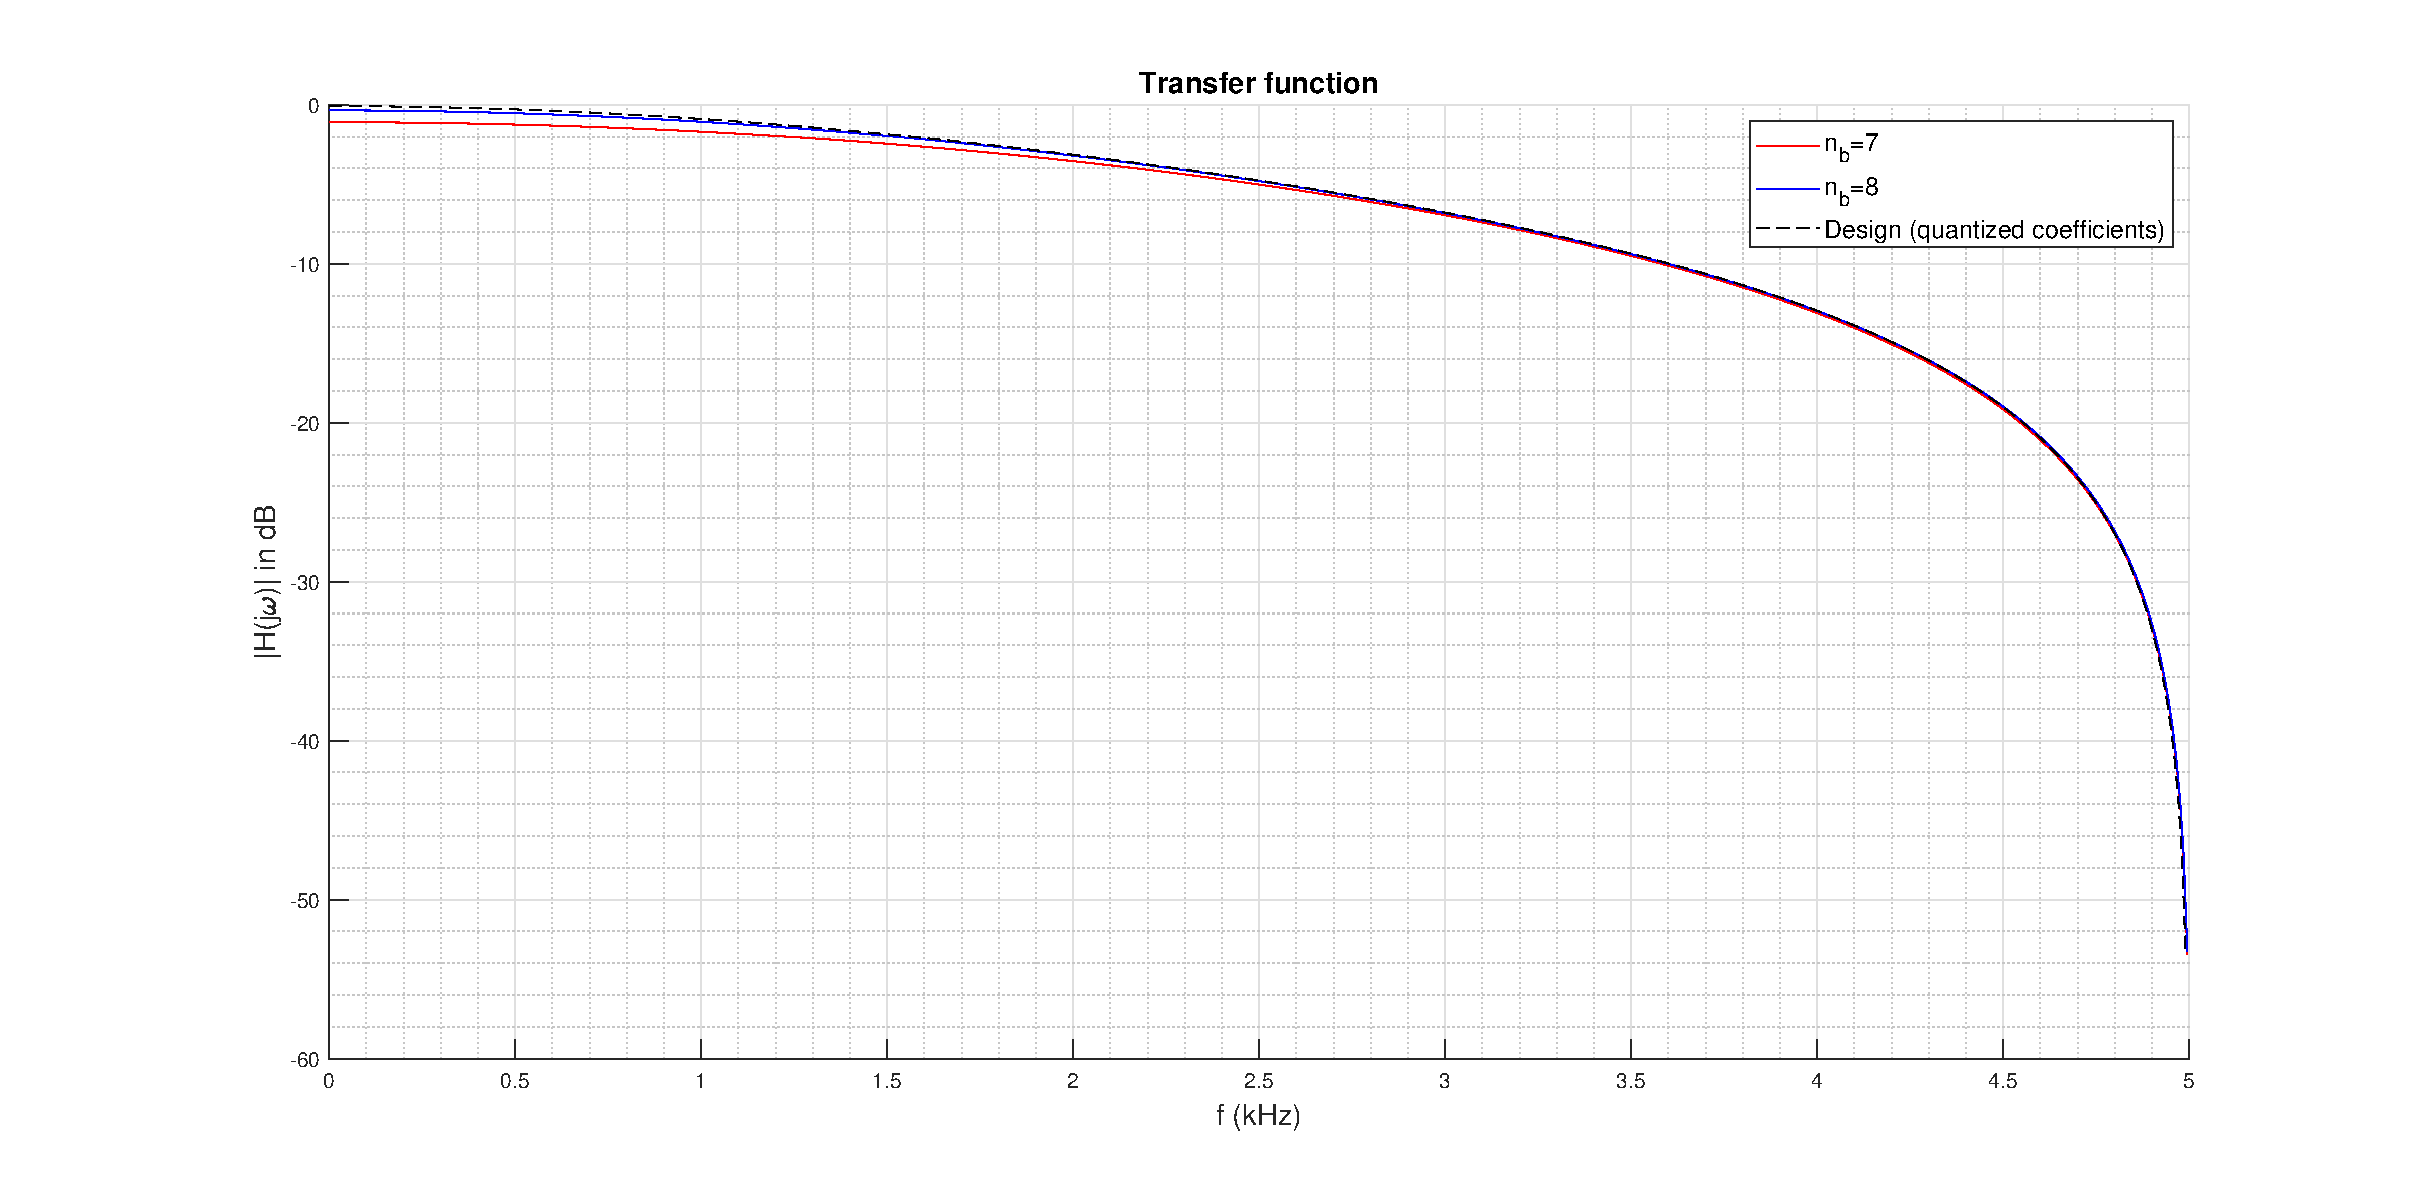
\includegraphics[width=1.4\textwidth]{./chapter1/images/tf_comparison.eps}}
	\caption{Transfer function for a few values of $n_b$}
	\label{fig:tfcomparison}
\end{figure}
\begin{figure}[htbp]
	\centering
	\makebox[\textwidth][c]{
	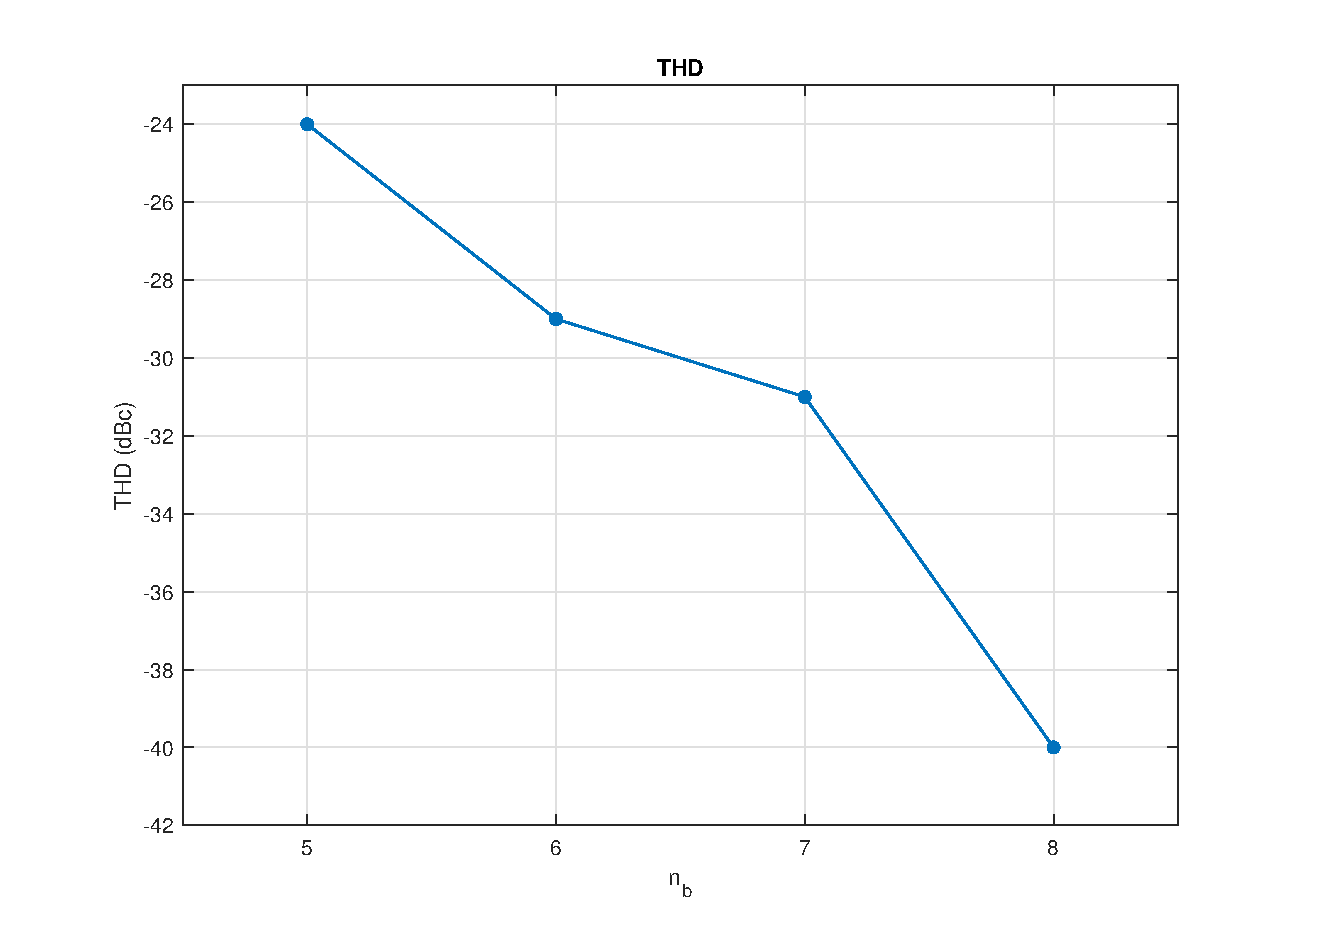
\includegraphics[width=1.4\textwidth]{./chapter1/images/thdplot.eps}}
	\caption{THD as a function of $n_b$}
	\label{fig:thdplot}
\end{figure}

\subsection{Datapath}
The datapath has been derived directly from the DFG in figure \autoref{fig:iir-dfd}. The specified timing requires to sample the incoming data in the same clock period where VIN is asserted. This is achieved by placing a register (\texttt{R1}) that latches the input at every clock cycle. Only valid inputs should be processed by the filter, therefore a latch is inserted in cascade at the output of \texttt{R1}. The latch enable is driven by the control unit so that the content of the input register is presented to the actual filter only when the input sample is valid. On the contrary, as long as VIN='0' the latch performs a gating function preventing the invalid content of the first register from reaching the filter. In this way, data registers within the filter need to be initialized to zero during the reset phase but do not need an enable signal because all internal values are held constant by the latch until a new samples is available.